\section{Einleitung}
Waren über das Internet zu bestellen ist heutzutage nichts außergewöhnliches mehr. Die Anzahl von Neueinsteigern im E-Commerce steigt. Dies verstärkt den Wettbewerb und führt dazu dass Unternehmen ihren E-Shop eine kontinuierlichen Optimierung unterziehen müssen. Kennzahlen unterstützten dabei das Auffinden von Schwachstellen und deren Ursachen. Dabei ist zu evaluieren welche Kennzahlen einen Mehrwert liefern und welche nicht. Die Gefahr zu viele Kennzahlen zu analysieren und dadurch den Blick für das Wesentliche zu verlieren ist groß.
Zu Beginn dieser Seminararbeit soll die Motivation, für den Einsatz von Kennzahlen zur Erfolgsmessung geweckt werden. Der aktuelle Forschungsstand und die gebildete Forschungsfrage, sollen den Rahmen für diese Arbeit definieren. Bevor sich dem Thema der Kennzahlen gewidmet wird, ist es erforderlich ein Verständnis für das Vorgehen im Web-Controlling zu erlangen. Zwei zentrale Aspekte sind zum einen der Web-Controlling Regelkreis und zum anderen die Konversionspfad-Analyse. Für dieses Vorgehen werden die resultierenden Chancen und Risiken aufgezeigt. Im Anschluss werden typische E-Shop Kennzahlen vorgestellt, die einerseits für die Erfolgsmessung genutzt werden, aber anderseits auch Schwachstellen und Optimierungspotenzial für die Erfolgstseigerung eines E-Shops aufweisen.

\subsection{Motivation}

\begin{figure}[H]
	\begin{center}
		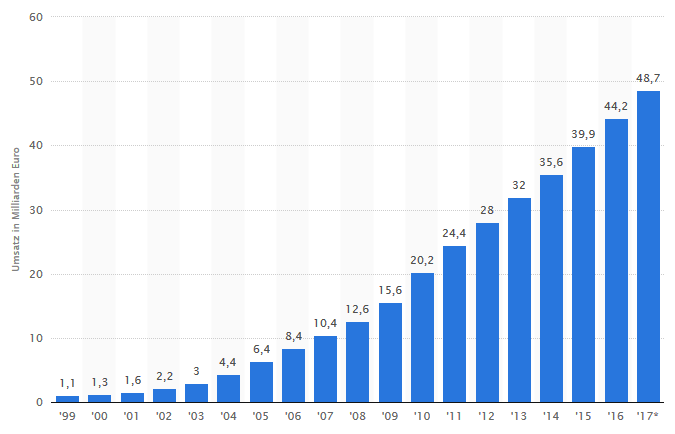
\includegraphics[width=0.9\textwidth]{umsatz}
		\caption{Umsatz durch E-Commerce (B2C) in Deutschland in den Jahren 1999 bis 2016 sowie eine Prognose für 2017 (in Milliarden Euro)~\footcite[Vgl. ][]{website:statista:umsatz}}
	\end{center}
\end{figure}

Der Umsatz der durch den elektronischen Handel in Deutschland generiert wird wächst kontinuierlich. Doch der Wettbewerb wird zusätzlich verstärkt durch Preissuchmaschinen und Bewertungsportale, die potenziellen Käufern die Möglichkeit bieten die Preise verschiedener Anbieter miteinander zu vergleichen~\footcite[Vgl. ][]{website:welt:artikel}. Dies führt zu sinkenden Margen und hören Kosten in der Kundenakquisition. Damit steigt auch die Relevanz für die Überwachung der eigenen Schwachstellen im eShop. Durch eine Analyse des eigenen E-Shop lässt sich das Kundenverhalten analysieren, welches wiederum ermöglicht Problem frühzeitig zu erkennen und Maßnahmen einzuleiten zur Erfolgssteigerung~\footcite[Vgl. ][Seite 36-37]{Hassler.2010}. Obwohl die Vorteile durch Einsatz von Kennzahlen offensichtlich sind, existieren noch erhebliche defizite in der Umsetzung~\footcite[Vgl. ][Seite 3, 8, 10]{website:unifreiburg:webanalytics}. In der Praxis besteht die Gefahr zu viele und wenige relevante Indikatoren zu analysieren. Daher empfiehlt Reese eine Zweck erfüllende Analyse des Nutzerverhaltens~\footcite[Vgl. ][Seite 42]{Reese.2009}. 

\subsection{Froschungsstand}
Die Analyse von Kennzahlen die speziell für die Erfolgsmessung eines E-Shops definiert werden, gewinnen in der Forschung immer mehr an Bedeutung~\footcite[Vgl. ][Seite 1]{Hienerth.2010}. Einer Studie zufolge ist die Praxiserfahrung jedoch noch gering und die Potenziale werden aktuell noch nicht vollumfänglich ausgeschöpft~\footcite[Vgl. ][Seite 9, 15]{website:unifreiburg:webanalytics}. Dabei ist zu beachten, dass hier eine Abgrenzung zum eigentlichen Web Analytics konstruiert wird. Der Begriff E-Shop Analytics wird in der Literatur dabei häufig genannt. Dieser versteht sich als ein Bestandteil des Web Analytics. Wie aus dem Namen bereits hervorgeht liegt der Fokus dabei auf der Analyse von E-Shops. Für diese spezielle Kategorie mangelt es aber noch an empirischen Studien~\footcite[Vgl. ][Seite 5]{website:unifreiburg:webanalytics2}.

\subsection{Forschungsfrage}
Mit Bezug auf das Kapitel 1.1 ist festzuhalten, dass die Vorteile einer Shopanalyse den Online-Händlern bekannt ist. Diese Potenziale werden aktuell noch nicht ausgeschöpft. Daraus leitet sich die Forschungsfrage dieser Seminararbeit ab:

Wie und mit welchen Kennzahlen, kann eine Erfolgsmessung durchgeführt werden, mit der eine Steuerung eines E-Shop möglich ist?

Das oberste Ziel eines E-Shops ist dabei immer der gleiche, nämlich der Absatz von Produkten und Dienstleistungen. Unter dieser Prämisse steht die Auswahl der betrachteten Kennzahlen. Um den Umfang dieser Seminararbeit zu begrenzen wird lediglich Bezug auf E-Shops im B2C-Umfeld genommen.

